\documentclass{article}
\usepackage[utf8]{inputenc}
\usepackage{listings}
\usepackage{color}

\definecolor{dkgreen}{rgb}{0,0.6,0}
\definecolor{gray}{rgb}{0.5,0.5,0.5}
\definecolor{mauve}{rgb}{0.58,0,0.82}


\lstset{frame=tb,
  language=python,
  aboveskip=3mm,
  belowskip=3mm,
  showstringspaces=false,
  columns=flexible,
  basicstyle={\small\ttfamily},
  numbers=none,
  numberstyle=\tiny\color{gray},
  keywordstyle=\color{blue},
  commentstyle=\color{dkgreen},
  stringstyle=\color{mauve},
  breaklines=true,
  breakatwhitespace=true,
  tabsize=3
}

\title{tem}
\author{Jason Guan }
\date{May 2017}

\usepackage{natbib}
\usepackage{graphicx}

\begin{document}

\maketitle

\section{Introduction}

\begin{lstlisting}
// Hello.java
import javax.swing.JApplet;
import java.awt.Graphics;

public class Hello extends JApplet {
    public void paintComponent(Graphics g) {
        g.drawString("Hello, world!", 65, 95);
    }    
}
\end{lstlisting}

\begin{figure}[h!]
\centering
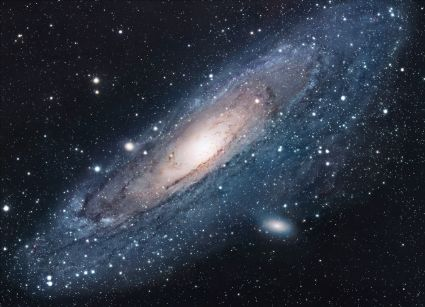
\includegraphics[scale=1.7]{universe.jpg}
\caption{The Universe}
\label{fig:univerise}
\end{figure}

\section{DNN - Udacity Section 2 lecture 9}
\subsection{Multilayer Neural Network}
ReLU
\subsection{Practice TensorFlow ReLUs}

\begin{lstlisting}
// python
hidden_layer = tf.add(tf.matmul(features, hidden_weights), hidden_biases)
hidden_layer = tf.nn.relu(hidden_layer)
output = tf.add(tf.matmul(hidden_layer, output_weights), output_biases)
\end{lstlisting}

\subsection{Tensorflow DNN}
\begin{lstlisting}
# input the dataset
from tensorflow.examples.tutorials.mnist import input_data
mnist = input_data.read_data_sets(".", one_hot=True, reshape=False)

# hyperparameter
import tensorflow as tf

learning_rate = 0.001
training_epochs = 20 # time of iteration
batch_size = 128  # lower this size if your memory is not enough
display_step = 1

n_input = 784   # MNIST data input, image size is 28*28
n_classes = 10  # MNIST total classes, total classes is 0-9 digits

# parameter in hidden_layer, which is the width of the layer
n_hidden_layer = 256

# weights and biases

weights = {
	'hidden_layer':tf.Variable(tf.random_normal((n_input, n_hidden_layer))),
	'out':tf.Variable(tf.random_normal((n_hidden_layer, n_classes)))
}
biases = {
	'hidden_layer':tf.Variable(tf.zeros(n_hidden_layer)), 
	# tf.zeros should always take a vector or matrix as input? can a scalar work
	'out':tf.Variable(tf.zeros(n_classes))
}

# input part
x = tf.placeholder('float', [None, 28, 28, 1])  # why there is always a None
y = tf.placeholder('float', [None, n_classes])

x_flat = tf.reshape(x, [-1, n_input])  # convert a 28 * 28 matrix to a 784 * 1 vector

# multilayer inceptron
layer_1 = tf.add(tf.matmul(x_flat, weights['hidden_layer']), biases['hidden_layer'])
layer_1 = tf.add(tf.matmul(layer_1, weights['out']), biases['out'])

logits = tf.add(tf.matmul(layer_1, weights['out']), biases['out'])

# Optimizer
cost = tf.reduce_mean(tf.nn.softmax_cross_entropy_with_logits(logits=logits, labels=y))
optimizer = tf.train.GradientDescentOptimizer(learning_rate=learning_rate).minimize(cost)

# Session
init = tf.global_variables_initializer()

with tf.Session() as sess:
	sess.run(init)
	
	for epoch in range(training_epochs):
		total_batch = int(mnist.train.num_examples/batch_size)
		for i in range(total_batch):
			# the method is provided by mnist
			batch_x, batch_y = mnist.train.next_batch(batch_size)  
			# but how do they feed the dict x and y to optimizer?
			sess.run(optimizer, feed_dict={x: batch_x, y: batch_y})

\end{lstlisting}

\subsection{About the Hidden Layer: why deeper not wider}

\begin{enumerate}
	\item Deep structure offers less parameters to estimate.
	\item Deep structure is compatible with the abstraction learning pattern of image recognition.
\end{enumerate}

\subsection{Save Tensorflow Model and Restore it}

\begin{lstlisting}
# remove previous tensors and operations
tf.reset_default_graph()

from tensorflow.examples.tutorials.mnist import input_data
import numpy as np

# Hyperparameter 
learning_rate = 0.001
n_input = 784
n_classes = 10

# Load dataset
mnist = input_data.read_data_sets('.', one_hot=True)

# Features and labels
features = tf.placeholder(tf.float32, [None, n_input])
labels = tf.placeholder(tf.float32, [None, n_classes])

# Weights and biases
# it is possible to trigger InvalidArgumentError: Assign requires shapes of both tensors to match.
# the name of tensor is better to be set explicitly 
weights = tf.Variable(tf.random_normal([n_input, n_classes]), name='weights')
biases = tf.Variable(tf.zeros([n_classes]), name='biases')

# Loss and optimizer
cost = tf.reduce_mean(tf.nn.softmax_cross_entropy_with_logits(logits=logits, labels=labels))
optimizer = tf.train.GradientDescentOptimizer(learning_rate=learning_rate).minimize(cost)

# Calculate accuracy
correct_prediction = tf.equal(tf.argmax(logits, 1), tf.argmax(labels, 1))
accuracy = tf.reduce_mean(tf.cast(correct_prediction, tf.float32))

# Train model and save weights
import math

save_file = './train_mode.ckpt'
batch_size = 128
n_epochs = 100

saver = tf.train.Saver()

with tf.Session() as sess:
	sess.run(tf.global_variables_initializer())
	
	# Loop over all batches
	for epoch in range(n_epochs):
		total_batch = math.ceil(mnist.train.num_examples / batch_size)
		
		for i in range(total_batch):
			batch_features, batch_labels = mnist.train.next_batch(batch_size)
			sess.run(optimizer, feed_dict={features: batch_features, labels: batch_labels})

		# Print status for every 10 epochs
		if epoch % 10 == 0:
			valid_accuracy = sess.run(
				accuracy, 
				feed_dict={features: mnist.validation.images, labels: mnist.validation.labels})
			print('Epoch {:<3} - Validation Accuracy: {}'.format(epoch, valid_accuracy))

	saver.save(sess, save_file)
	print('Trained Model Saved.')

saver = tf.train.Saver()

with tf.Session() as sess:
	saver.restore(sess, save_file)
	test_accuracy = sess.run(accuracy, feed_dict={features: mnist.test.images, labels:mnist.test.labels})

print('Test Accuracy:{}'.format(test_accuracy))
\end{lstlisting}

\subsection{Regularization}

\begin{enumerate}
	\item Early Termination
	Stop to train as soon as the validation set performance begins to slide down.
	\item L2 Regularization
	$$ L' = L + \beta \frac{1}{2} ||\omega||_{2}^2 $$
	
\end{enumerate}

\section{Conclusion}
``I always thought something was fundamentally wrong with the universe'' \citep{adams1995hitchhiker}

\bibliographystyle{plain}
\bibliography{references}
\end{document}
